\documentclass[11pt,a4paper]{article}
\usepackage[T1]{fontenc}
\usepackage[utf8]{inputenc}
\usepackage[margin=1in]{geometry}
\usepackage{graphicx}
\usepackage{booktabs}
\usepackage{array}
\usepackage{amsmath,amssymb}
\usepackage{enumitem}
\usepackage{hyperref}
\usepackage{listings}
\usepackage{xcolor}
\usepackage{float}
\usepackage{placeins}
\usepackage{fancyhdr}

\graphicspath{{docs/}}

\hypersetup{
  colorlinks=true,
  linkcolor=blue,
  urlcolor=blue,
  citecolor=blue,
  hypertexnames=false
}

\setlength{\parindent}{0pt}
\setlength{\parskip}{0.6em}
\setlength{\headheight}{15pt}
\setlist[itemize]{leftmargin=1.4em}
\setlist[enumerate]{leftmargin=1.4em}

\newcolumntype{L}[1]{>{\raggedright\arraybackslash}p{#1}}

\lstset{
  basicstyle=\ttfamily\small,
  breaklines=true,
  frame=single,
  columns=fullflexible,
  showstringspaces=false,
  keepspaces=true
}

\renewcommand{\sectionmark}[1]{\markright{\thesection\ #1}}
\renewcommand{\subsectionmark}[1]{\markright{\thesubsection\ #1}}

\pagestyle{fancy}
\fancyhf{}
\fancyhead[L]{\small BandDPER}
\fancyhead[C]{\nouppercase{\large\bfseries \rightmark}}
\fancyfoot[L]{\small Mathieu WAHARTE}
\fancyfoot[C]{\thepage}
\fancyfoot[R]{\small April 2026}
\renewcommand{\headrulewidth}{0.4pt}
\renewcommand{\footrulewidth}{0.4pt}

\fancypagestyle{plain}{%
  \fancyhf{}
  \fancyhead[L]{\small BandDPER}
  \fancyhead[C]{\nouppercase{\large\bfseries \rightmark}}
  \fancyfoot[L]{\small Mathieu WAHARTE}
  \fancyfoot[C]{\thepage}
  \fancyfoot[R]{\small April 2026}
  \renewcommand{\headrulewidth}{0.4pt}
  \renewcommand{\footrulewidth}{0.4pt}
}

\title{BandDPER\\\large Band-Aware Dual-Perspective Equivariant ResNet}
\author{Mathieu WAHARTE}
\date{April 2026}

\begin{document}

\maketitle
\tableofcontents

\clearpage
\begin{figure}[p]
  \centering
  
\includegraphics[width=\textwidth,height=0.85\textheight,keepaspectratio]{dual_perspective_flowchart.png}
  \caption{Model architecture flowchart for BandDPER.}
  \label{fig:model-architecture-flowchart}
\end{figure}
\FloatBarrier

\clearpage
\section{Analysis}

\subsection{Problem Statement}
Since the game is a full-information, deterministic, zero-sum game with a small board ($6\times6$) and a fixed topology but non uniform (the band map), we can leverage strong domain knowledge to design an efficient and effective evaluation function. The key challenge is to capture the complex interactions between pieces, the band constraints (creates strong local dependencies between adjacent squares), and the strategic patterns that emerge from the unique movement rules.

\subsection{Requirements}
First, we can be certain that the evaluation function should return a scalar in $[-1, +1]$, where -1 represents a losing position for the current player, +1 represents a winning position, and values in between represent varying degrees of advantage.

The function must capture several key signals:
\begin{itemize}
  \item Which pieces can legally move right now (band constraint)
  \item How many moves each side has (mobility asymmetry)
  \item Proximity of attackers to the opponent's unicorn, weighted by band alignment and measured in a unicorn-relative coordinate frame
  \item Unicorn escape routes (counted explicitly as scalar signal)
  \item Structural patterns (corridor control, band-type distribution)
  \item Tempo forcing: which band the current move lands on determines the opponent's forced departure
  \item Forced-pass detection: whether the current move leaves the opponent with no legal response
\end{itemize}

\subsection{Why a Neural Network}
Compared to our handcrafted evaluation function which already captures the most obvious signals, a neural network can learn nonlinear interactions, generalize easily from training data and capture structural patterns that were not encoded in our formula.
The main drawback is that it would be slower but according to \href{https://arxiv.org/abs/1712.01815}{AlphaZero}, a better evaluation with a shallower depth can outperform a deeper search with a worse evaluation. Furthermore, the game is very small ($6\times6$ with 12 pieces) and networks are heavily researched and inference optimizations can make it nearly as fast as a handcrafted eval.

\newpage
\subsection{Existing Models}
\begin{table}[htbp]
  \centering
  \begin{tabular}{L{0.12\textwidth} L{0.53\textwidth} L{0.27\textwidth}}
    \toprule
    Model & Notes & Recommendation \\
    \midrule
    MLP & Fast & No spatial awareness or relational reasoning, avoid \\
    CNN & Exploits local spatial patterns and translation equivariance; fast enough & Ok but overkill; translation equivariance may be wrong \\
    NNUE & Fast incremental updates, dual-perspective design, ClippedReLU (-1 to 1) activation & Doesn't fit current problem size, but dual-perspective, ClippedReLU, king-relative features, and direct output shortcuts are interesting ideas to borrow \\
    ResNet & Good if baseline evaluation exists & Good, but lacks inherent spatial awareness \\
    GNN & Movement graph; invariant to symmetries & Avoid due to dynamic graph changes, complexity, and slower performance \\
    \bottomrule
  \end{tabular}
    \caption{Existing model candidates and recommendations.}
    \label{tab:existing-models}
\end{table}

\clearpage
\section{Model Architecture}

This architecture blends known components into a novel evaluation network:
\begin{itemize}
  \item \textbf{Siamese CNN spatial encoder} with shared weights and dual-perspective input
  \item \textbf{Band topology and game signals encoded as fixed and dynamic input channels} (16 channels total)
  \item \textbf{Unicorn-relative attacker map} inspired by NNUE's HalfKP king-relative encoding
  \item \textbf{Residual trunk} with ClippedReLU at the perspective boundary
  \item \textbf{Scalar injection} of escape counts at the trunk boundary
  \item \textbf{Direct output shortcut} for forced-pass signal, bypassing the trunk
\end{itemize}

Core design elements:
\begin{itemize}
  \item \textbf{Siamese Network} (Shared-weight dual-perspective encoding, \href{https://papers.nips.cc/paper/1993/hash/0d4262ad58b4d3866d5aa0f4f9e1c06b-Abstract.html}{Bromley et al. - 1993})
  \item \textbf{ResNet} (CNN + residual blocks, \href{https://arxiv.org/abs/1512.03385}{He et al. - 2015})
  \item \textbf{Atrous convolution} (Dilated convolutions for range, \href{https://arxiv.org/abs/1511.07122}{Chen et al. - 2015})
  \item \textbf{ClippedReLU} bounded activations (\href{https://official-stockfish.github.io/docs/nnue-pytorch-wiki/docs/nnue.html}{NNUE - 2018})
  \item \textbf{Dual accumulator} for game positions (\href{https://official-stockfish.github.io/docs/nnue-pytorch-wiki/docs/nnue.html}{NNUE - 2018})
  \item \textbf{Unicorn-relative encoding} inspired by HalfKP king-relative features (\href{https://official-stockfish.github.io/docs/nnue-pytorch-wiki/docs/nnue.html}{NNUE - 2018})
  \item \textbf{Direct output shortcut} for near-linear signals (\href{https://github.com/official-stockfish/Stockfish/blob/master/src/nnue/nnue_architecture.h}{Stockfish HalfKAv2 PSQT bypass - 2021})
  \item \textbf{Value head} (Value network for board games, \href{https://arxiv.org/abs/1712.01815}{AlphaZero - 2017})
\end{itemize}

\textbf{Parameter Count}
\begin{table}[htbp]
  \centering
  \caption{Approximate parameter count by component.}
  \label{tab:parameter-count}
  \begin{tabular}{L{0.58\textwidth} L{0.25\textwidth}}
    \toprule
    Component & Parameters \\
    \midrule
    Encoder (shared, used $\times2$) & $\sim$312,000 \\
    ResBlock $\times3$ (dim=258) & $\sim$402,648 \\
    Output head & $\sim$16,577 \\
    \textbf{Total} & \textbf{$\sim$730,625} \\
    \bottomrule
  \end{tabular}
\end{table}

This model would be around 2.9 MB in float32.
The reduced variant with \texttt{embed\_dim=64}, \texttt{num\_res\_blocks=2} has around \textbf{185K parameters}.

\newpage
\subsection{Layers}

\subsubsection{Input}
For each perspective we have a $[16, 6, 6]$ tensor. For each board position, we have 16 channels:

\begin{table}[htbp]
  \centering
  \caption{Input channels for each perspective tensor.}
  \label{tab:input-channels}
  \begin{tabular}{L{0.10\textwidth} L{0.50\textwidth} L{0.28\textwidth}}
    \toprule
    Channel & Content & Type \\
    \midrule
    0 & My paladin positions & Dynamic 0/1 \\
    1 & My unicorn position & Dynamic 0/1 \\
    2 & Opponent paladin positions & Dynamic 0/1 \\
    3 & Opponent unicorn position & Dynamic 0/1 \\
    4 & Band-1 square mask & \textbf{Fixed} 0/1 \\
    5 & Band-2 square mask & \textbf{Fixed} 0/1 \\
    6 & Band-3 square mask & \textbf{Fixed} 0/1 \\
    7 & Departure constraint mask & Dynamic 0/1 \\
    8 & Band-1 legal landing squares & Dynamic 0/1 \\
    9 & Band-2 legal landing squares & Dynamic 0/1 \\
    10 & Band-3 legal landing squares & Dynamic 0/1 \\
    11 & My row occupancy fraction & Dynamic $[0,1]$ \\
    12 & Opponent row occupancy fraction & Dynamic $[0,1]$ \\
    13 & My column occupancy fraction & Dynamic $[0,1]$ \\
    14 & Opponent column occupancy fraction & Dynamic $[0,1]$ \\
    15 & Unicorn-relative opponent attacker map & Dynamic 0/1 \\
    \bottomrule
  \end{tabular}
\end{table}

\emph{Band masks (ch. 4--6) are fixed binary inputs representing the board's spatial structure.} \\
\emph{Channels 8--10 makes the tempo-forcing mechanic explicit.} \\
\emph{Channel 15 places opponent paladins in a coordinate frame centered on our unicorn (anchor at row=2, col=2), inspired by HalfKP's king-relative encoding. This lets the CNN learn threat patterns that are translation-invariant relative to the unicorn.}

This encodes the full current board state.
The CNN will learn the spatial correlations between pieces and band types.
Having two perspectives allows us to follow the \textbf{Siamese network principle}, where the same encoder processes both perspectives with shared weights, enabling the network to learn a unified representation of the game state from both players' viewpoints. Indeed, a position that is good for one player is bad for the other (menacing the unicorn is universally bad), so the network can learn to extract features that are relevant for both sides without needing separate encoders.

In addition, \textbf{3 scalars are injected} outside the CNN:
\begin{table}[htbp]
  \centering
  \caption{Scalar injections.}
  \begin{tabular}{L{0.20\textwidth} L{0.45\textwidth} L{0.25\textwidth}}
    \toprule
    Scalar & Content & Injection point \\
    \midrule
    \texttt{escape\_me} & Legal move count for my unicorn (0--16) & Concatenated into \texttt{h} \\
    \texttt{escape\_opp} & Legal move count for opponent unicorn & Concatenated into \texttt{h} \\
    \texttt{forced\_pass} & 1 if opponent has no legal reply & Direct output bypass \\
    \bottomrule
  \end{tabular}
\end{table}

The escape counts are appended to \texttt{h} after Siamese fusion.
The forced-pass bit bypasses the trunk entirely as a learned additive weight on the output scalar.

\newpage
\subsubsection{Shared Spatial Encoder}
\begin{figure}[H]
  \centering
  
\includegraphics[width=\textwidth,height=0.80\textheight,keepaspectratio]{SSE.png}
  \caption{Shared Spatial Encoder used for both player perspectives (shared weights).}
  \label{fig:shared-spatial-encoder}
\end{figure}
\FloatBarrier

Figure~\ref{fig:shared-spatial-encoder} details the encoder stack used to extract perspective-specific embeddings. With $B$ the batch size.

\textbf{Notes}:
\begin{itemize}
  \item The first convolution captures \textbf{local spatial patterns} and piece interactions, which are crucial for evaluating immediate threats and opportunities. Its receptive field of $3\times3$ allows it to see adjacent pieces and band types. Importantly, broken-path movement of band=2 pieces reaches exactly the diagonal neighbours captured by this $3\times3$ kernel - so this convolution is now the primary movement-range detector.
  \item The second convolution with dilation=2 \textbf{expands the receptive field} (effective $5\times5$) to capture medium-range interactions such as L shaped movement patterns and corridor control.
  \item \textbf{BatchNorm}: Applied after each convolution to stabilize training and accelerate convergence.
  \item \textbf{ClippedReLU}: Used in the encoder output to ensure all values are in the range $[0,1]$, preventing one perspective from dominating the other due to scale differences.
  \item \textbf{Dual-Perspective Fusion}: The outputs from both perspectives are concatenated to form a unified representation \texttt{h} of shape $[B, 256]$, then escape counts are appended giving \texttt{h} shape $[B, 258]$. Always pass inputs in the order \texttt{[current\_player, opponent]}.
  \item Both perspectives are processed through the same encoder (shared weights) to learn a unified representation of the game state, enabling the network to generalize patterns that are relevant for both players (Siamese network principle).
\end{itemize}

\newpage
\subsubsection{Residual Trunk}
There is a trunk of 3 ResBlocks with skip connections. Each ResBlock consists of:

\begin{figure}[H]
  \centering
  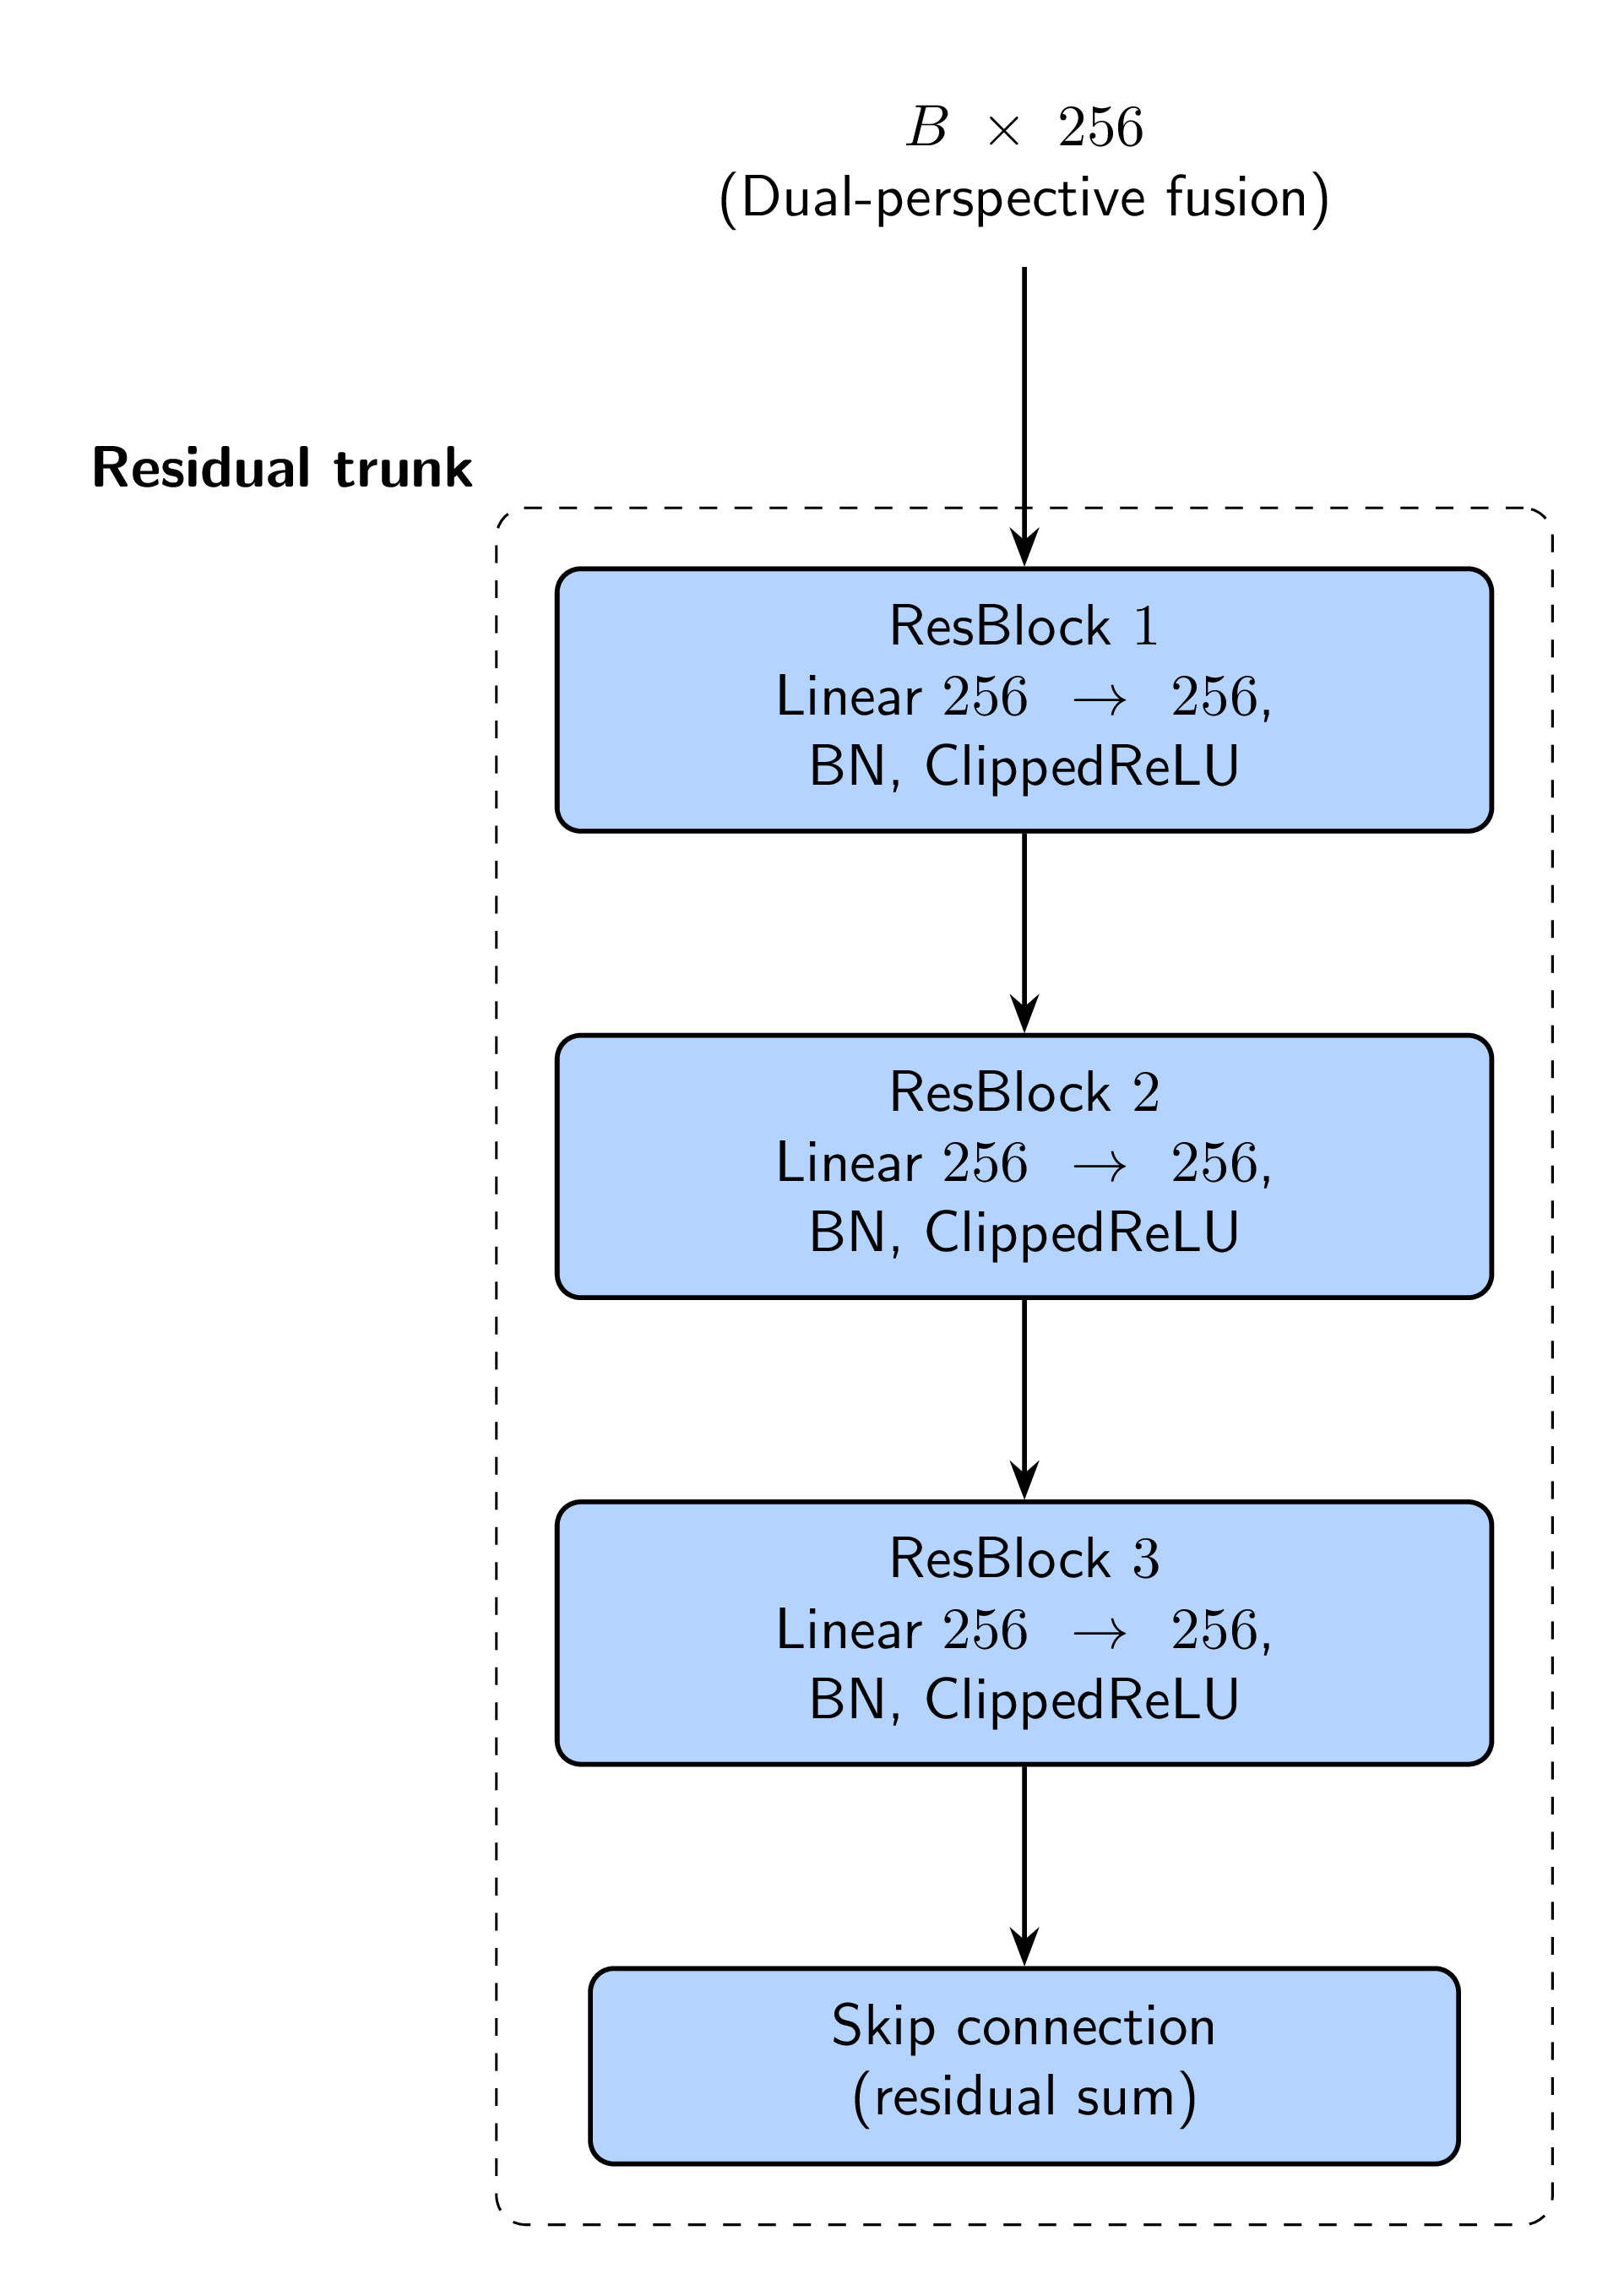
\includegraphics[width=\textwidth,height=0.58\textheight,keepaspectratio]{residual_trunk.png}
  \caption{Residual trunk structure with stacked ResBlocks and skip connections.}
  \label{fig:residual-trunk}
\end{figure}
\FloatBarrier

Figure~\ref{fig:residual-trunk} shows the repeated residual pattern used to refine the fused representation.

A residual block computes an output $y$ as the sum of its input $x$ and a learned function $F(x)$: $y = F(x) + x$.
The function $F$ is typically a small neural network (e.g., two linear layers with an activation in between).
This structure allows the block to learn a residual function (essentially a correction to its input) rather than needing to learn a full transformation from scratch.
Additionally, the skip connection (the ``$+x$'' part) allows gradients to flow directly through the block during backpropagation, which helps mitigate the vanishing gradient problem and enables training of deeper networks.
This also provides graceful degradation as, if a block learns to output zero (i.e., $F(x) \approx 0$), it effectively becomes an identity function, allowing the network to skip it without harming performance.

\textbf{Input dimension}: 258 (256 Siamese CNN output + 2 escape scalars).

\newpage
\textbf{Notes}:
\begin{itemize}
  \item \textbf{Why residual blocks}: The network learns \emph{corrections} on top of a near-correct base representation. This is the right structure when training via minimax bootstrapping. Skip connections prevent vanishing gradients with depth.
  \item \textbf{Why 3 ResBlocks}: Maps to Escampe's three natural abstraction levels (proximity/unicorn-relative $<$ band interaction/tempo $<$ forced-pass/escape dynamics). Matches empirical optimum from board game literature at this parameter scale (\href{https://en.wikipedia.org/wiki/AlphaZero}{AlphaZero}, \href{https://arxiv.org/pdf/2107.08387}{Train on Small, Play the Large: scaling up board games with AlphaZero and GNN}, \href{https://arxiv.org/html/2409.12272v1#S6}{Mastering Chess with a Transformer Model}). A smaller block count wouldn't capture the full complexity of this game and going to three blocks is worth the additional cost. Also, with ClippedReLU, more than 3 blocks would lead to training instability as the gradient path through the skip connections becomes dominant and the $F(x)$ branch receives progressively weaker gradients. Meaning wise, after 3 levels of composition, further blocks learn redundant representations since the positional complexity is fundamentally bounded by the board size and piece interactions.
  \item \textbf{Why ClippedReLU in ResBlocks}: Keeps activations bounded at every depth, preventing value explosion through skip connections.
  \item \textbf{Scalar injection at trunk input}: Escape counts are global signals that do not have a natural spatial representation. Injecting them at \texttt{h} (after the CNN, before the trunk) lets the ResBlocks learn to combine spatial features with game-state scalars. The trunk's Linear($258\to258$) layer learns the projection automatically.
\end{itemize}

\newpage
\subsubsection{Output Head}
The output head uses a direct bypass for forced pass signals, inspired by \href{https://github.com/official-stockfish/Stockfish/blob/master/src/nnue/nnue_architecture.h}{Stockfish's PSQT direct-to-output shortcut}:

\begin{figure}[H]
  \centering
  
\includegraphics[width=\textwidth,height=0.34\textheight,keepaspectratio]{output_head.png}
  \caption{Output head producing a bounded scalar evaluation.}
  \label{fig:output-head}
\end{figure}
\FloatBarrier

\texttt{w\_pass} is a single learned scalar parameter. Wiring the forced pass signal directly to the output bypasses the trunk entirely, giving this near-linear signal maximum gradient and preventing the trunk from having to learn to route it.

This mirrors Stockfish HalfKAv2's \texttt{FullThreats} feature set, which is passed directly to the output layer for a similar reason - some signals have a nearly linear effect on evaluation, and the hidden layers add noise rather than value.

No ClippedReLU on the output since Tanh already bounds the final value. The output is a scalar representing the evaluation from the current player's perspective.

\clearpage
\section{Training}

\subsection{Data Generation (Minimax Bootstrapping)}
We use the \textbf{existing alpha-beta engine} at depth 4--6 to label positions with ``ground truth'' scores.
The network learns to approximate deep search evaluations.
Precisely, for each position sampled from self-play games, we run a minimax search to get the score and use it as the training label: \texttt{score\_label = minimax(board, depth=5) / MATE\_SCORE} (normalized to $[-1,1]$).
This is a form of supervised learning where the target labels are generated by a stronger search algorithm.
We aim at around 50K--100K labeled positions, which is sufficient for the network to learn meaningful patterns without overfitting.

\textbf{Note on the band constraint and forced pass signals}: Both require knowing the last move's landing band, not just the board position. Ensure training examples store \texttt{(board\_state, last\_landing\_band, label)} triples, not just \texttt{(board\_state, label)}. Forced-pass positions are rare ($\sim$2--5\% of positions); the direct shortcut ensures they receive strong gradient despite low frequency.

Alternatively, we could use \textbf{TD-learning} but minimax bootstrapping is more straightforward and effective for our purposes.

\subsection{Loss Function}
We use \textbf{Mean Squared Error} (MSE) loss between the network's predicted score and the minimax score label:

\begin{lstlisting}[language=Python]
loss = F.mse_loss(prediction, target)
\end{lstlisting}

\subsection{Optimizer and Training Hyperparameters}
We use \textbf{AdamW} (\texttt{lr=1e-3}, \texttt{weight\_decay=1e-4}) with \textbf{Cosine Annealing with Warm Restarts} to escape plateaus during iterative bootstrapping rounds. We also apply \textbf{gradient clipping} (\texttt{clip\_grad\_norm\_=1.0}) to prevent exploding gradients.

\subsection{Training Hardware}
We used a GTX 1080 GPU for training, which is more than sufficient for this model size and dataset.

\begin{lstlisting}[language=bash]
pip install torch torchvision --index-url https://download.pytorch.org/whl/cu118
\end{lstlisting}

\newpage
\subsection{Export Pipeline}
\begin{lstlisting}[language=Python]
# 1. Fold BatchNorm into conv/linear weights (eliminates BN at inference)
def fold_batchnorm(w, b, bn_mean, bn_var, bn_gamma, bn_beta, eps=1e-5):
  std = (bn_var + eps).sqrt()
  return w * (bn_gamma/std).view(-1,1,1,1), \
      bn_gamma*(b-bn_mean)/std + bn_beta

model = fold_all_batchnorms(model)

# 2. Export all weights to JSON (include w_pass and new band masks)
weights = {k: v.tolist() for k,v in model.state_dict().items()}
weights["band1_mask"] = BAND1_MASK.tolist()
weights["band2_mask"] = BAND2_MASK.tolist()
weights["band3_mask"] = BAND3_MASK.tolist()
weights["w_forced_pass"] = model.w_forced_pass.item()  # w_pass weight
json.dump(weights, open("escampe_net_weights.json","w"))

# 3. Save .pth for resuming training
torch.save(model.state_dict(), "escampe_net.pth")

# 4. Push to HuggingFace
api.upload_file("escampe_net.pth",
                path_in_repo="escampe_net.pth",
                repo_id="mathieu-waharte/escampe-eval")
\end{lstlisting}

\clearpage
\section{Inference}

We load the weights once at startup, then run forward pass manually:

\begin{lstlisting}[language=Java]
// Pre-allocate all activation buffers (no GC pressure in hot path)
float[][][] convBuf1, convBuf2;
float[]     encBuf, wEmbed, bEmbed, trunk, h1, outBuf;
float       wForcedPass;   // w_pass: loaded once at startup

public float evaluate(EscampeBoard board, int lastLandingBand) {
  float[][][] xMe  = boardToTensor(board, board.currentPlayer(), lastLandingBand);
  float[][][] xOpp = boardToTensor(board, board.opponent(),      lastLandingBand);

  float[] w = encode(xMe);   // [128], ClippedReLU output
  float[] b = encode(xOpp);  // [128]

  // Scalar signals: escape counts, normalized to [0,1]
  float escapeMe  = computeUnicornEscapeCount(board, board.currentPlayer()) / 16.0f;
  float escapeOpp = computeUnicornEscapeCount(board, board.opponent())      / 16.0f;

  // Concatenate perspectives + escape scalars [258]
  float[] h = concat(w, b, new float[]{escapeMe, escapeOpp});

  // ResBlocks
  for (ResBlockWeights rb : resBlocks) {
    h = resBlock(h, rb);
  }

  // Output head
  float[] out = linear(h, wOut1, bOut1);  // [64]
  out = relu(out);
  float raw = linear(out, wOut2, bOut2)[0];  // [1]

  // Forced-pass: direct output shortcut, bypasses trunk
  int forcedPass = computeForcedPass(board, lastLandingBand);
  raw += wForcedPass * forcedPass;

  return (float) Math.tanh(raw);
}
\end{lstlisting}

\clearpage
\section{Optimizations}

\subsection{Masks, maps and channels}
Band masks, departure masks, band-landing maps, row/column occupancy maps, unicorn-relative attacker maps, escape scalars, and the forced-pass direct shortcut are the strongest low-cost inductive bias improvements for our setting. They provide the network with explicit information about the board's spatial structure, piece interactions, and game-specific mechanics that are critical for learning effective evaluations.
We are currently using the following inputs:
\begin{itemize}
  \item Row/column occupancy maps (channels 11--14)
  \item Band-landing maps (channels 8--10)
  \item Unicorn escape counts (scalars at \texttt{h})
  \item Forced-pass direct shortcut (scalar at output)
  \item Unicorn-relative attacker map (channel 15)
\end{itemize}

\subsection{Iterative re-bootstrap rounds}
After training the initial network, we can use it to generate new labels by running a deeper minimax search (depth 6--8) with the network as its evaluation function. This iterative bootstrapping is a key technique used in AlphaZero.

\subsection{Weighted value loss}
We can modify the MSE loss to give more weight to positions that are closer to winning or losing.

\subsection{SE blocks}
Squeeze-and-Excitation blocks can be added after convolutional layers to allow the network to learn channel-wise attention. Lightweight and easily integrated.

\subsection{Depthwise separable convolutions}
Replacing standard convolutions in the encoder with depthwise separable convolutions can reduce parameters and computational cost while maintaining performance.

\subsection{Policy head for move ordering}
We propose adding a \textbf{policy head} that outputs a probability distribution over the $\sim$96 possible moves (up from $\sim$60 under straight-line movement, due to broken-path movement reaching more destinations per band: 4/8/16 unique destinations for band 1/2/3 respectively from interior squares). Used purely for move ordering in alpha-beta search.

\begin{lstlisting}[language=Python]
policy_head = nn.Sequential(
    Linear(258, 64),
    ReLU(),
    Linear(64, 96),
    Softmax(dim=-1)
)
\end{lstlisting}

Then for each node in the search tree:
\begin{enumerate}
  \item Generate legal moves (existing move generator, very fast)
  \item Call the policy head to get move probabilities and sort moves once per node (slower but improves pruning)
  \item Run alpha-beta with well-ordered moves for better pruning
  \item Use handcrafted eval at leaf nodes \textbf{/!\textbackslash} unless network inference is fast enough
\end{enumerate}

\subsection{Quantization}
\begin{table}[htbp]
  \centering
  \caption{Quantization choices by layer.}
  \label{tab:quantization-choices}
  \begin{tabular}{L{0.30\textwidth} L{0.12\textwidth} L{0.16\textwidth} L{0.30\textwidth}}
    \toprule
    Layer & Params & Quantize? & Why \\
    \midrule
    Conv layers (encoder) & $\sim$33K & INT8 & Weights are small, well-distributed \\
    Linear proj ($2688\to32$) & $\sim$86K & INT8 & Biggest layer, most to gain \\
    ResBlock linears & $\sim$8K & INT8 & Clean after ClippedReLU \\
    Output Linear($64\to1$) & 65 & keep float32 & Tiny, output precision matters \\
    \texttt{w\_forced\_pass} & 1 & keep float32 & Single scalar, precision matters \\
    Band mask channels & fixed & N/A & Already binary (0/1) \\
    \bottomrule
  \end{tabular}
\end{table}

In ONNX/PyTorch:
\begin{lstlisting}[language=Python]
model.eval()
model_q = torch.quantization.quantize_dynamic(
  model,
  {nn.Linear, nn.Conv2d},
  dtype=torch.qint8
)
torch.onnx.export(model_q, (x_w, x_b, esc_me, esc_opp, forced_pass),
                  "escampe_net_q8.onnx")
\end{lstlisting}

And in Java with ONNX Runtime:
\begin{lstlisting}[language=Java]
// pom.xml: com.microsoft.onnxruntime:onnxruntime:1.17.0
OrtEnvironment env = OrtEnvironment.getEnvironment();
OrtSession session = env.createSession("escampe_net_q8.onnx");
// ~1-2us inference for 25K param INT8 model via ONNX Runtime
\end{lstlisting}

To evaluate the quantization performance, we propose to compare the score predictions of the quantized model against the original float32 model on a large set of random board positions. We then compute the mean absolute error (MAE) and mean squared error (MSE) between the two sets of predictions with 95, 99, 99.99 confidence intervals (to check if edge cases don't get degraded). Additionally, we can run a small tournament of 1000 self-play games using both models as evaluation functions in the search, and compare their win rates to see if the quantization has a significant impact on playing strength.


\subsection{Distillation}
Train a smaller ``student'' network to mimic the outputs of the larger ``teacher'' network using KL divergence + MSE distillation loss.\\
\href{https://arxiv.org/html/2503.13178}{Rapfi: Distilling Efficient Neural Network for the Game of Gomoku}

\subsection{Rejected optimizations}
\begin{itemize}
  \item \textbf{$1\times6/6\times1$ asymmetric kernels}: Were originally considered to capture row/column patterns due to a missunderstanding of the movement rules. However, with broken-path movement, pieces can reach both orthogonal and diagonal neighbours, so a standard $3\times3$ kernel is more appropriate to capture all local interactions.
  \item \textbf{Attention pooling / self-attention in encoder}: Conflicts with incremental-style updates, global interaction cost excessive for board size.
  \item \textbf{NNUE-style incremental updates}: Architecture is convolutional and not naturally NNUE-like.
  \item \textbf{LayerNorm replacing folded BatchNorm}: Export pipeline folds BatchNorm away at inference.
  \item \textbf{Pre-activation ResNet}: Too little upside for only 3 residual blocks.
  \item \textbf{DenseNet-style dense connections}: Memory overhead without obvious benefit.
  \item \textbf{Full transformerization}: Too expensive and poorly matched for latency target and board size.
\end{itemize}

\clearpage
\section{References}

\subsection{Papers and architecture references}
\begin{itemize}
  \item \href{https://papers.nips.cc/paper/1993/hash/0d4262ad58b4d3866d5aa0f4f9e1c06b-Abstract.html}{Bromley et al. - 1993}: Siamese network / shared-weight dual-perspective encoding
  \item \href{https://arxiv.org/abs/1512.03385}{He et al. - 2015}: ResNet residual blocks
  \item \href{https://arxiv.org/abs/1511.07122}{Chen et al. - 2015}: Atrous (dilated) convolutions
  \item \href{https://arxiv.org/abs/1712.01815}{AlphaZero - 2017}: Value head and improved evaluation via search
  \item \href{https://arxiv.org/pdf/2107.08387}{Train on Small, Play the Large: scaling up board games with AlphaZero and GNN}: Small-board AlphaZero scaling
  \item \href{https://arxiv.org/html/2409.12272v1#S6}{Mastering Chess with a Transformer Model}: Transformer-based chess scaling insights
  \item \href{https://official-stockfish.github.io/docs/nnue-pytorch-wiki/docs/nnue.html}{NNUE - 2018}: ClippedReLU, dual accumulator, HalfKP king-relative features, direct output shortcuts
  \item \href{https://github.com/official-stockfish/Stockfish/blob/master/src/nnue/nnue_architecture.h}{Stockfish HalfKAv2 architecture}: FullThreats direct-to-output connection (source of J shortcut idea)
  \item \href{https://www.chessprogramming.org/Stockfish_NNUE}{Stockfish NNUE - Chessprogramming wiki}: HalfKP/HalfKAv2 feature set design rationale
  \item \href{https://arxiv.org/html/2503.13178}{Rapfi: Distilling Efficient Neural Network for the Game of Gomoku}: Distillation techniques for board game evaluation networks
\end{itemize}

\subsection{Tools and implementation references}
\begin{itemize}
  \item \href{https://download.pytorch.org/whl/cu118}{PyTorch CUDA 11.8 wheels}: GPU build used for training on GTX 1080
  \item \href{https://onnxruntime.ai}{ONNX Runtime}: Inference engine referenced for quantized model execution
\end{itemize}

\end{document}